\chapter{実装}
\label{chap:developing}
本章では, Delta Smile Facial Survey Analyzer の実装部分について説明する.
まずユーザーインターフェースの実装について説明し, システム全体の画面遷移の流れを最初に示す.
次にデータ収集機能の各モジュールの実装について整理し, データ分析機能の各モジュールの実装について
説明し,まとめる.

\section{ユーザーインターフェースの実装}
本システムではおよそ3分程度で一連のデータ収集機能のシステム処理を行う.
開発言語はpythonを使用し, バージョンは3.6.1 を使用した.
実行コマンドは以下のように行う. mode\_num は0を引数に指定するとユーザーからのデータを収集し,
1を指定すると既存の動画に対して処理を行いデータ形成を行うことできる.

\begin{itemize}
\item 実行コマンド
\begin{lstlisting}
$ python dsfsa.py mode_num
\end{lstlisting}
%複数の時は以下のように
%\item 実行コマンド
%\begin{lstlisting}
%$ python dsfsa.py mode_num
%\end{lstlisting}
\end{itemize}

ユーザーに見せるシーンとして全部で8種類のシーンが存在する.
各シーンは全てオープンソースのOpenCVを使用して, ディスプレイeizo sx2761wに表示をしている.
それぞれの表示内容, 役割について以下に述べる.

\subsection{ユーザーインターフェースシーン1}
図\ref{fig:seen1}のシーン1はシステムを起動した最初のシーンである.
実験の際に, 個人情報である表情のデータを使うため, ユーザーの同意が必要である.
パソコンのReturnキーを一回入力することで実験, データ提供への同意を得るように実装を行った.

\subsection{ユーザーインターフェースシーン2}
図\ref{fig:seen2}のシーン2はユーザーの基本情報を収集するためのシーンである.
基本情報として, 性別と年齢を何十歳の形で入力をする.
入力したデータは.txtファイルとしてユーザーごとのフォルダーに保存するようにした.

\subsection{ユーザーインターフェースシーン3}
図\ref{fig:seen2}のシーン2にて,基本情報を入力したのちに, 図\ref{fig:seen3}のシーン3へ自動で遷移する.
このシーンでは実際にユーザーの映像がwebカメラ,Logicool C920r の映像が映し出される.
遷移と同時にカメラに映る一番大きな顔をユーザーの顔として認識をしトラッキングを行っている.

\subsection{ユーザーインターフェースシーン4}
図\ref{fig:seen4}のシーン4では, 図\ref{fig:seen3}のシーン3にて, 笑顔が検出された場合にはユーザーの笑顔が検出されていることを知らせる
小さいウィンドウが表示され, 検出した口元に緑色の長方形が描画されるようになっている.

\subsection{ユーザーインターフェースシーン5}
図\ref{fig:seen4}のシーン4にて, 笑顔が一定フレーム以上検出された後, 図\ref{fig:seen5} のシーン5へ移動する.
シーン5が表示されている間にフレーム分析処理, 動画作成処理, データ選択処理が行われており,
およそ20秒ほど処理を待機する時間が発生する.

\subsection{ユーザーインターフェースシーン6}
図\ref{fig:seen6}のシーン6はユーザーから入力を受け付けるシーンである.
点描画によって映し出されている笑顔動画データに対して順位づけを行う.
計5つ, 4回のキーボード入力を行い, 各笑顔動画データに対して順位づけデータを与える.

\subsection{ユーザーインターフェースシーン7}
図\ref{fig:seen7}のシーン7は結果表示画面であり, ユーザーの笑顔動画データを左側, 右側にユーザーが1番高く
順位づけした笑顔動画データを並列で表示する.

\subsection{ユーザーインターフェースシーン8}
図\ref{fig:seen8}のシーン8はシステム終了前のシーンである.
笑顔動画データベースおよび収集した笑顔動画データの中に含まれる全ての笑顔フレームを表示する.

\begin{figure}[htbp]
    \begin{center}
       \fbox{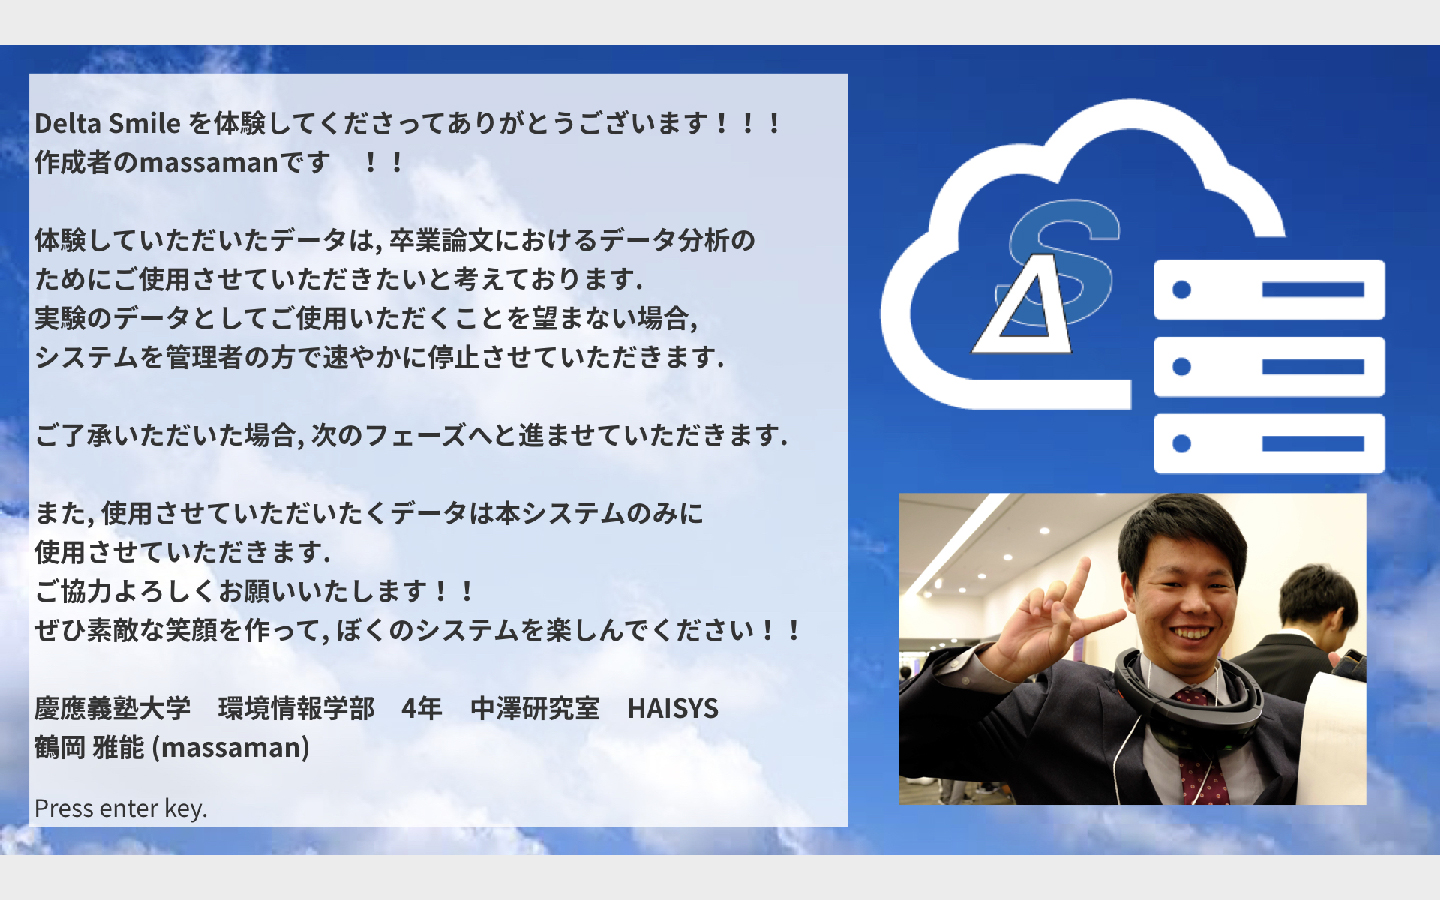
\includegraphics[width=140mm,bb=0 0 1440 900]{seen1.jpg}}
    \end{center}
    \caption{ユーザーインターフェースシーン1}
    \label{fig:seen1}
\end{figure}

\begin{figure}[htbp]
    \begin{center}
       \fbox{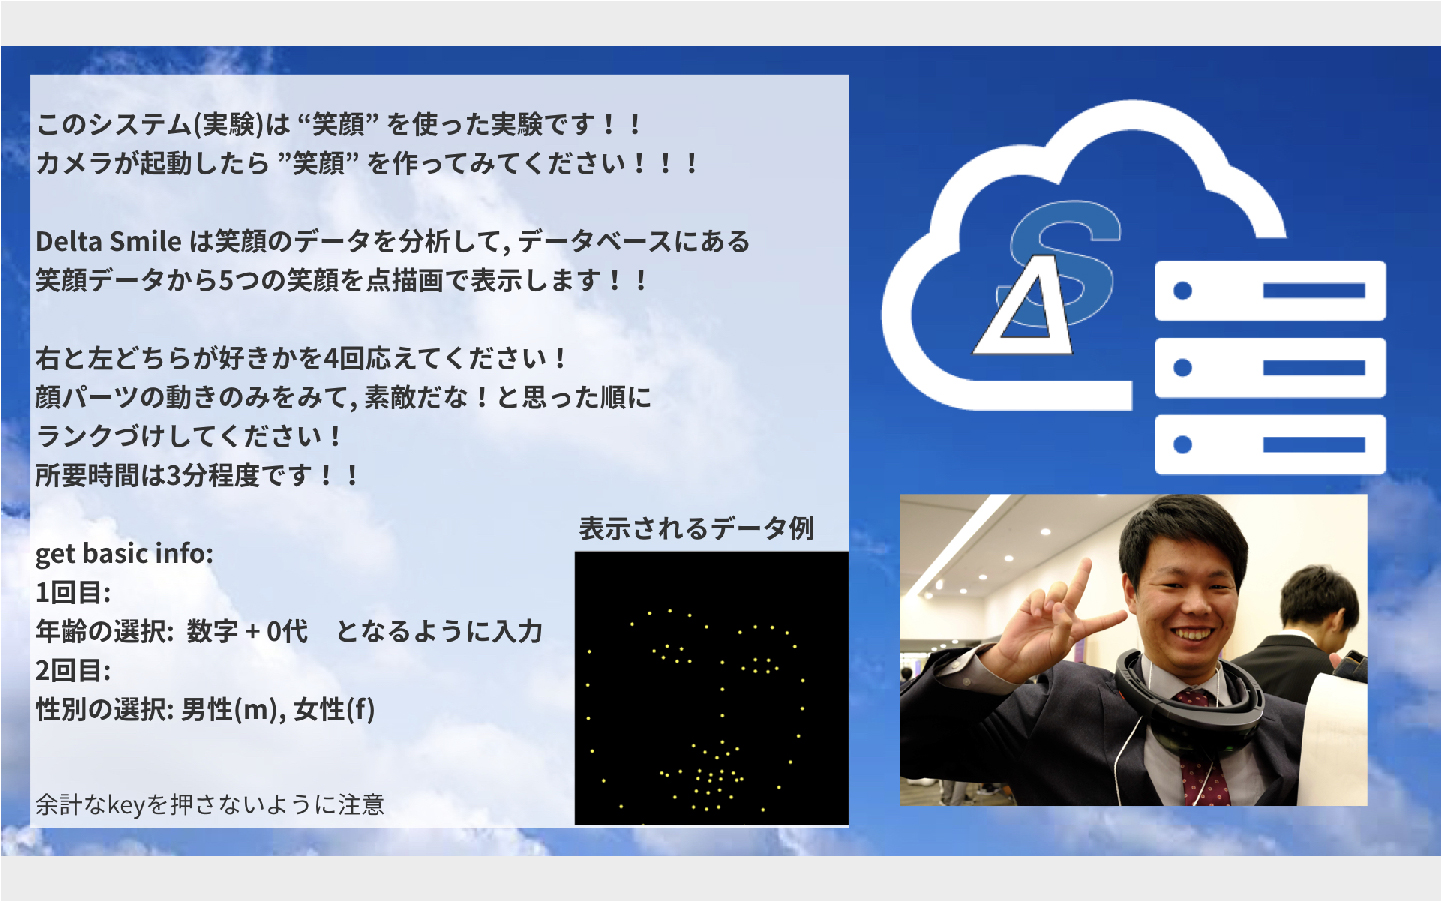
\includegraphics[width=140mm,bb=0 0 1440 900]{seen2.jpg}}
    \end{center}
    \caption{ユーザーインターフェースシーン2}
    \label{fig:seen2}
\end{figure}

\begin{figure}[htbp]
    \begin{center}
       \fbox{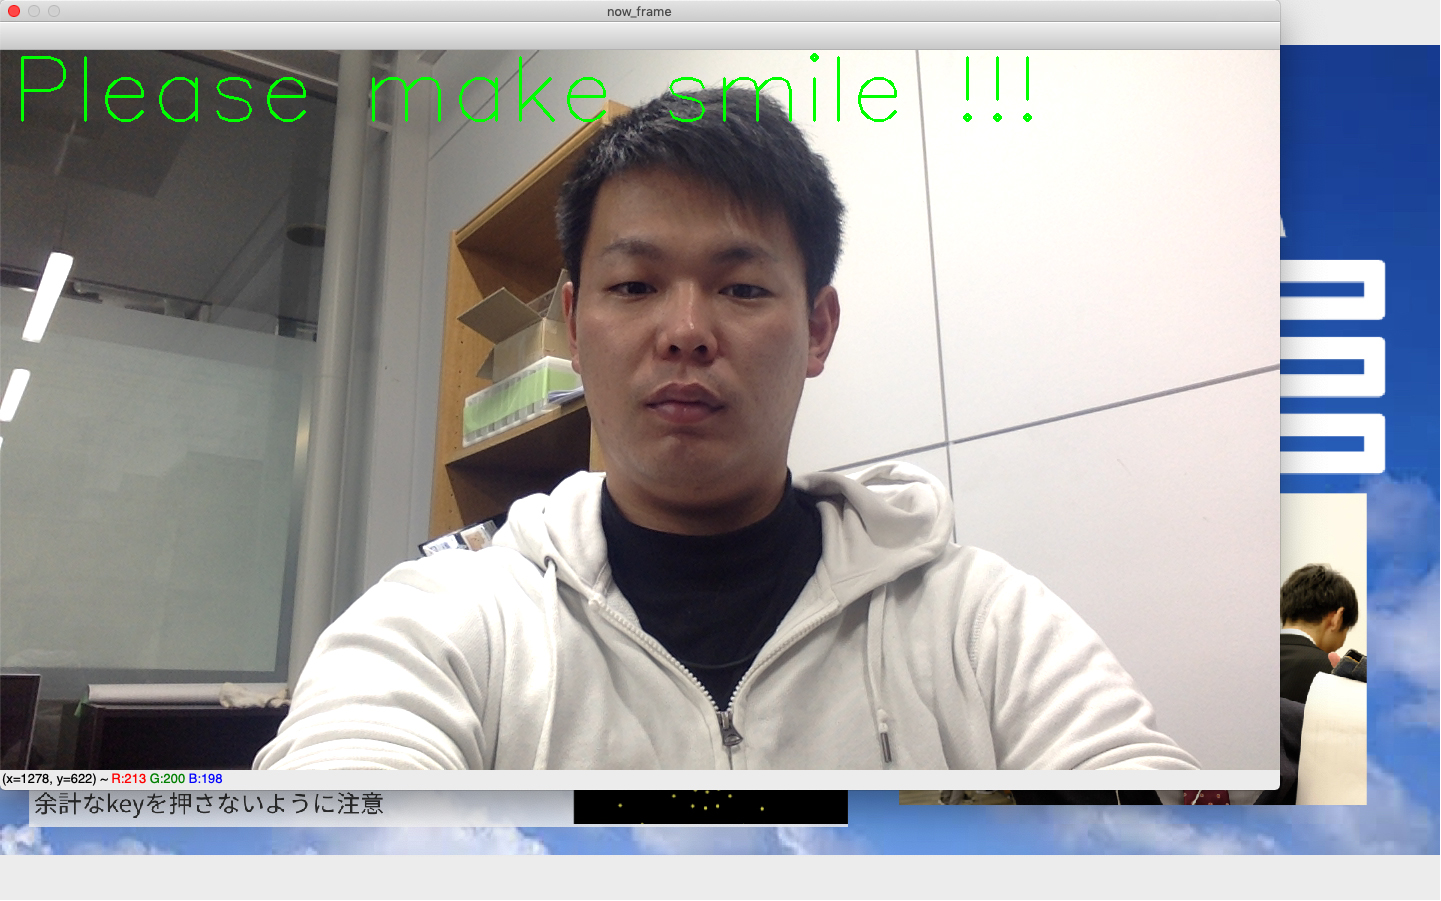
\includegraphics[width=140mm,bb=0 0 1440 900]{seen3.jpg}}
    \end{center}
    \caption{ユーザーインターフェースシーン3}
    \label{fig:seen3}
\end{figure}

\begin{figure}[htbp]
    \begin{center}
       \fbox{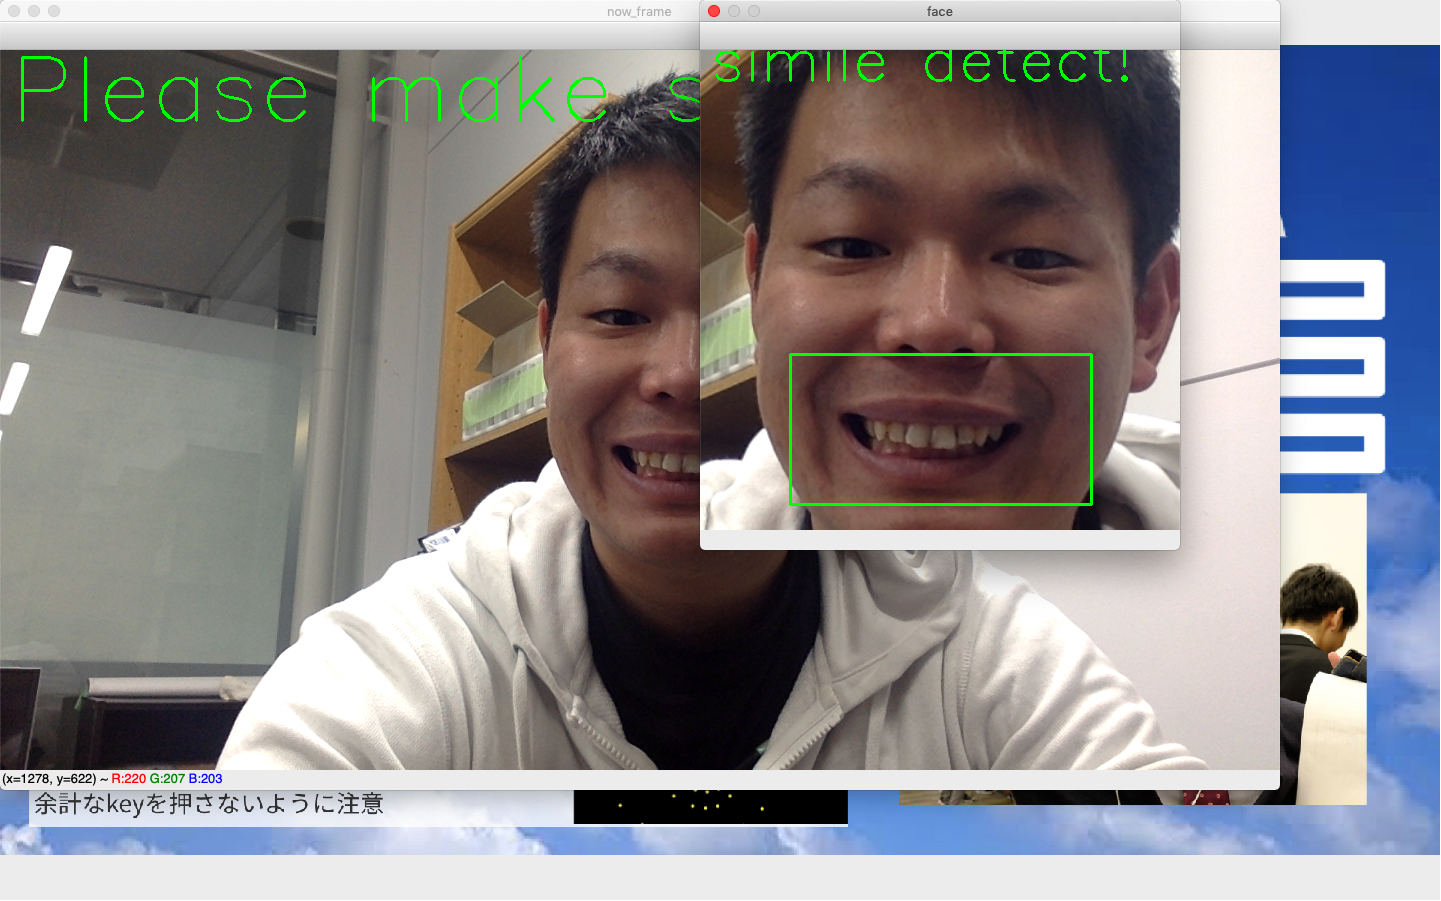
\includegraphics[width=140mm,bb=0 0 1440 900]{seen4.jpg}}
    \end{center}
    \caption{ユーザーインターフェースシーン4}
    \label{fig:seen4}
\end{figure}

\begin{figure}[htbp]
    \begin{center}
       \fbox{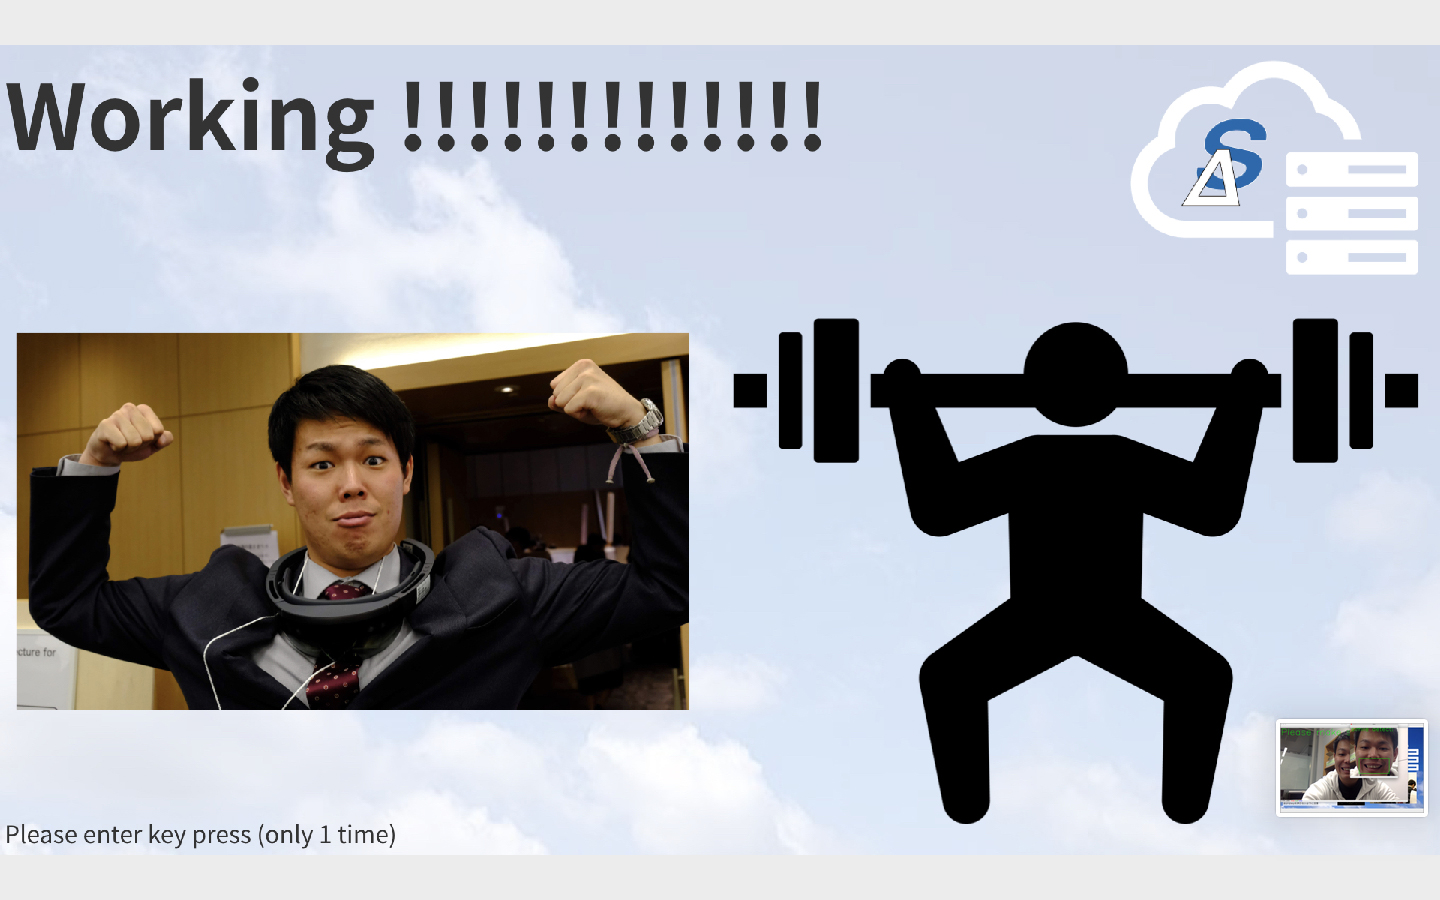
\includegraphics[width=140mm,bb=0 0 1440 900]{seen5.jpg}}
    \end{center}
    \caption{ユーザーインターフェースシーン5}
    \label{fig:seen5}
\end{figure}

\begin{figure}[htbp]
    \begin{center}
       \fbox{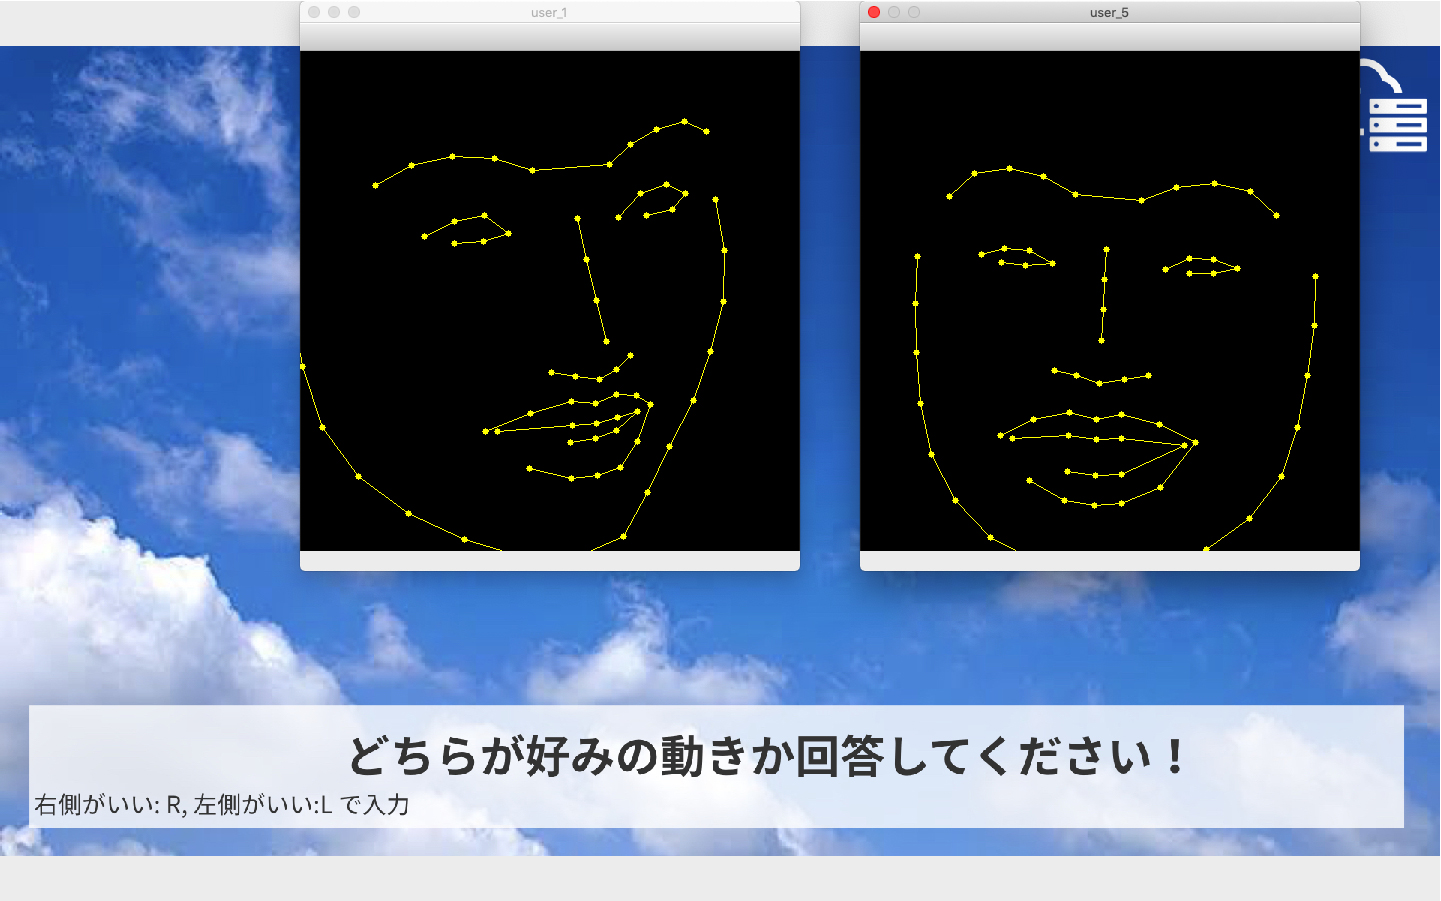
\includegraphics[width=140mm,bb=0 0 1440 900]{seen6.jpg}}
    \end{center}
    \caption{ユーザーインターフェースシーン6}
    \label{fig:seen6}
\end{figure}

\begin{figure}[htbp]
    \begin{center}
       \fbox{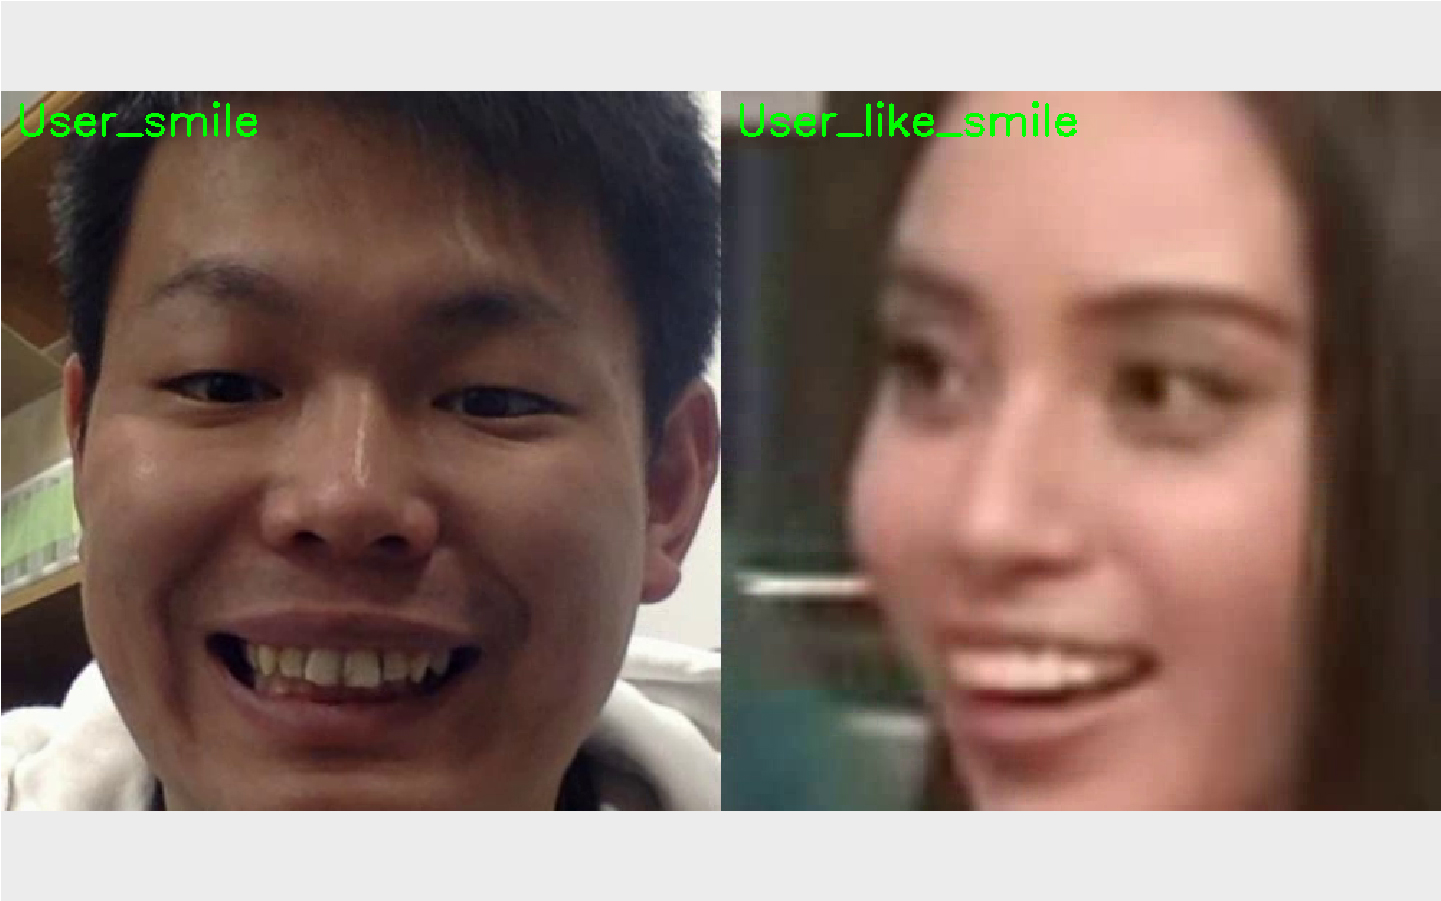
\includegraphics[width=140mm,bb=0 0 1440 900]{seen7.jpg}}
    \end{center}
    \caption{ユーザーインターフェースシーン7}
    \label{fig:seen7}
\end{figure}

\begin{figure}[htbp]
    \begin{center}
       \fbox{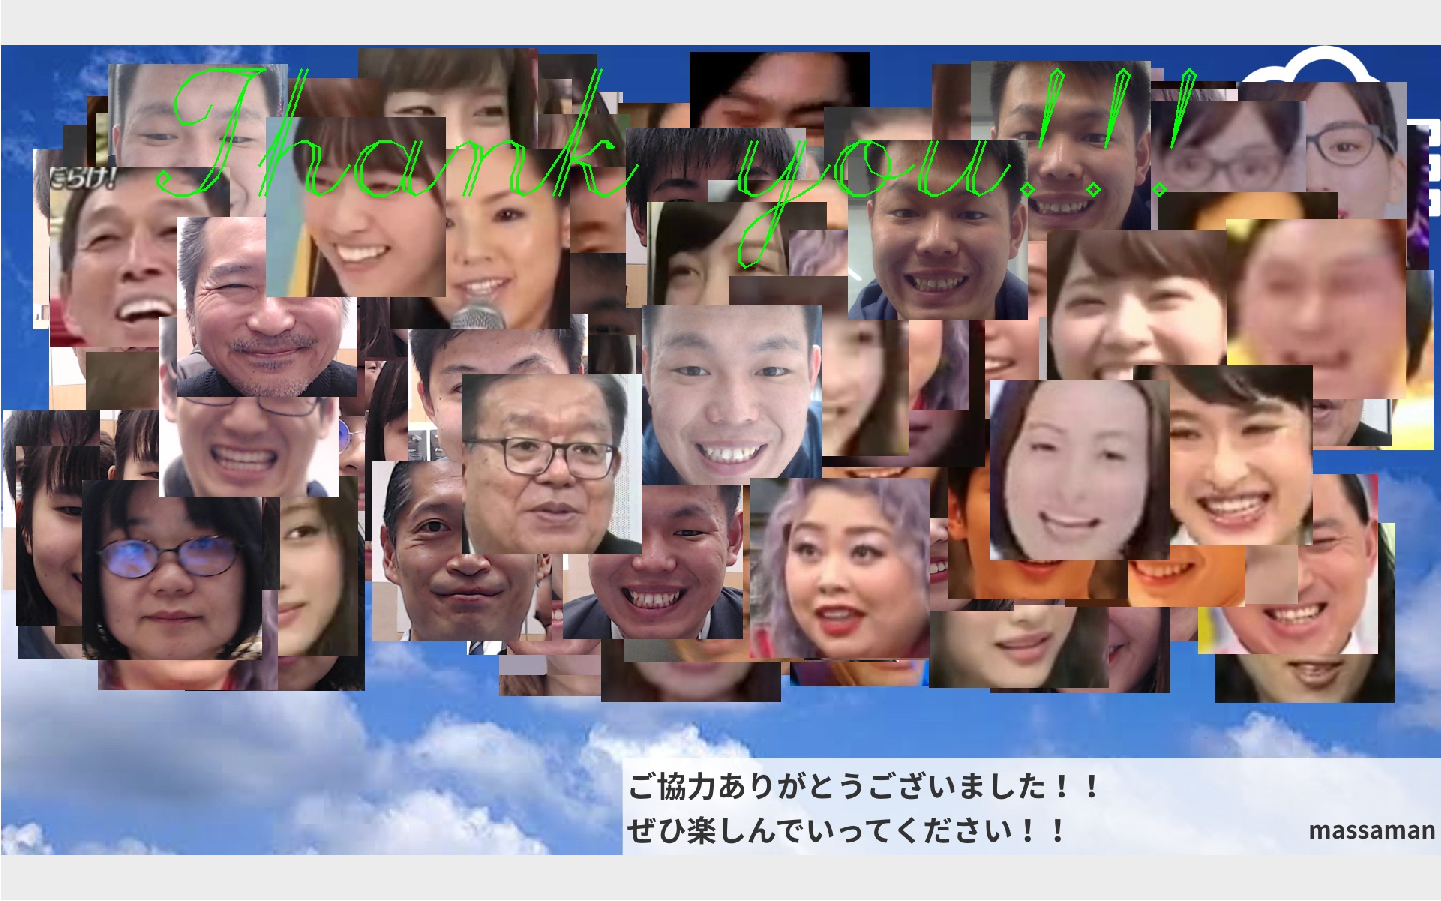
\includegraphics[width=140mm,bb=0 0 1440 900]{seen8.jpg}}
    \end{center}
    \caption{ユーザーインターフェースシーン8}
    \label{fig:seen8}
\end{figure}


\section{データ収集機能の実装}
このセクションでは, 各モジュールの実装の詳細について述べる.

\subsection{顔検出モジュールの実装}
顔検出はオープンソースであるOpenCVの中に含まれるカスケードである,
haarcascade\_frontalface\_default.xmlをOpenCVで読み込み使用する.
読み込んだ全ての動画フレームに対して顔検出の処理を行う.
\begin{itemize}
\item 顔検出検出パラメーター
\begin{lstlisting}
face_list =face_detect_cascade.detectMultiScale(
  gray,scaleFactor = 1.21,
  minNeighbors = 15,
  minSize=(300,300)
  )
\end{lstlisting}
\end{itemize}
検出した全ての動画フレームに対して表示処理を行う場合, システムのラグが発生するため,表示は偶数フレームのみとした.
返り値の画像に含まれる顔の左上のx座標およびy座標, 横幅と高さの値を次の関数へと引き継ぐ.

\subsection{笑顔検出モジュールの実装}
顔検出モジュールで得た返り値の値を参照し,顔のある領域のみに対して笑顔の検出処理を全てのフレームに対して行う.
笑顔の判別はOpenCVの中に含まれるhaarcascade\_smile.xmlを読み込み使用する.
このカスケードは顔の口の領域に対して処理を行い笑顔の検出を行う.
webカメラから取得した画像全ておよび, 全ての領域に対して笑顔検出の処理を行うことも可能であるが,
実装のテスト段階で誤検出が多かったため, 顔を検出しその中でも誤検出が一番少ないパラメータ調整を行った.

\begin{itemize}
\item 笑顔検出パラメーター
\begin{lstlisting}
smile_detector =smile_cascade.detectMultiScale(
  face_gray,scaleFactor= 1.7,
  minNeighbors=20,
  minSize=(120, 120)
  )
\end{lstlisting}
\end{itemize}

顔を検出したフレームが20フレーム以上,および笑顔を検出したフレームが5フレーム以上になった場合に
検出を終了する.

\subsection{画像処理モジュールの実装}
顔検出および笑顔検出モジュールで取得したフレームに対して, 画像処理を行う.
検出したフレームをコンパイルしたOpenFaceのFaceLandmarkImg関数を使用して, 全てのフレームから
顔のパーツの動きを表したFacial Action Unitの値をcsvファイルに算出する.
各フレームごとに生成されるため, ユーザーごとに1つのファイルにマージする処理をここで行う.

\begin{itemize}
\item OpenFace算出パラメータ例:
\begin{lstlisting}
frame, timestamp, confidence, success,
gaze_0_x, gaze_0_y, gaze_0_z, gaze_1_x, gaze_1_y, gaze_1_z,
pose_Tx, pose_Ty, pose_Tz, pose_Rx, pose_Ry, pose_Rz,
x_0, x_1, ... x_67, y_0, y_1, ..., y_67,
X_0, X_1,..., X_67, Y_0, Y_1,..., Y_67, Z_0, Z_1, ... Z_67,
p_scale, p_rx, p_ry, p_rz, p_tx, p_ty, p_0, p_1, ..., p_33,
AU01_r, AU02_r, AU04_r, AU05_r, AU06_r, AU09_r, AU10_r,
AU12_r, AU14_r, AU15_r, AU17_r, AU20_r, AU25_r, AU26_r,
AU04_c, AU12_c, AU15_c, AU23_c, AU28_c, AU45_c
\end{lstlisting}
\end{itemize}

\subsection{動画作成モジュールの実装}
フレームごとに処理をした後, 全てのフレームを時系列順に結合して笑顔動画データの作成を行う.
フレームには保存時にファイル名で時系列順に番号を振っており, 配列にデータを格納しソートすることで
時系列順に処理を行うことが可能である.
本システムにおいて,fps(Frame per Seconds) は20であったため1秒間の動画が生成される.

\subsection{データ作成モジュールの実装}
一番初めに入力したユーザーの基本データ, 画像処理モジュールで生成したCSVファイルおよび動画作成モジュール
で作成したユーザーの笑顔動画データをユーザーごとにファイリングしてデータフォーマットとする.
作成したデータは各ユーザーごと, 各データの種類ごとの2通りの方法でデータを保存する.

\subsection{笑顔動画データ選択モジュールの実装}
\subsection{表示データ作成モジュールの実装}
\subsection{順位づけモジュールの実装}
\subsection{データ保存モジュールの実装}
\subsection{選択データ表示モジュールの実装}

\section{データ分析機能の実装}
作成中...
\subsection{FAU値計算モジュールの実装}
\subsection{データプロットモジュールの実装}
\section{まとめ}
